\nofiles
\documentclass{acta}
\usepackage{supertabular,lscape,epsfig}
\usepackage{amssymb}
\usepackage{amsmath}
\usepackage{tikz}
\usetikzlibrary{positioning}

\SetPages{0}{0}

\SetVol{58}{2008}

\begin{document}


\begin{Titlepage}
\Title{The Mathematical Foundation of Astrometric Observation Geometry: A Review of SPICE Underlying Models}
\Author{J~a~s~o~n P.$^{1,*}$ \dots and K~a~l~a, I.$^2$}
{$^1$Department of Information Technology, Nehru Institute of Technology, Coimbatore, Tamil Nadu, India\\
e-mail: pandiajason@gmail.com\\
$^2$Department of Computer Science and Engineering, PSG Institute of Technology and Applied Research, Coimbatore, Tamil Nadu, India\\
$^*$Corresponding author}

\Received{Month Day, Year}
\end{Titlepage}

\Abstract{Modern astrometry and planetary science rely heavily on automated toolkits to map celestial coordinates, spacecraft trajectories, and instrument pointing vectors. While NASA's SPICE toolkit is universally adopted for this purpose, its underlying mathematical frameworks---spanning relativistic time transformations, non-linear interpolations, and quaternion algebra---are often treated as a ``black box'' by the observational community. This paper provides a rigorous mathematical survey of the foundational algorithms driving the SPICE kernels (SPK, PCK, CK, FK, and LSK). We explicitly derive the core vector transformation chains, evaluate the precision thresholds of different body-shape models (ellipsoids vs. tessellated meshes), and quantify how numerical truncation and interpolation choices propagate into milliarcsecond-level astrometric uncertainties. This survey serves as a standalone analytical reference for observational astronomers, astrometrists, and mission design engineers seeking to move beyond black-box software application and understand the mathematical foundation of modern observation geometry.}{astrometry -- celestial mechanics -- reference frames -- methods: analytical -- methods: numerical -- ephemerides}

\section{Introduction}
Modern observational astronomy and deep-space planetary exploration demand an unprecedented level of geometric precision. Estimating the coordinate-state of a distant spacecraft, aligning a telescope's instrument boresight with an asteroid, or mapping high-resolution spectrometer data onto a comet's surface requires a rigorous, consistent mathematical framework. For over three decades, the Spacecraft, Planet, Instrument, C-matrix, Events (SPICE) toolkit, developed and maintained by NASA's Navigation and Ancillary Information Facility (NAIF), has served as the international standard for calculating these complex geometric relationships (Acton 1996, Acton \etal 2018).

Despite its ubiquitous adoption, a significant portion of the astronomical community utilizes SPICE as an engineering black box. Astronomical papers frequently cite the software toolkit without detailing the underlying mathematical models, approximations, or coordinate systems. This practice poses a scientific risk, as observational geometry calculations are subject to physical constraints, numerical limits, and modeling approximations that directly impact scientific conclusions (Pajusalu \etal 2022). Furthermore, a point of minor confusion exists in interdisciplinary nomenclature: in electrical engineering, ``SPICE'' refers to the Simulation Program with Integrated Circuit Emphasis, a circuit simulation tool (Miranda 2024), whereas in observational astronomy and planetary science, SPICE represents the geometric information system designed by NAIF.

\begin{figure}[htb]
\begin{center}
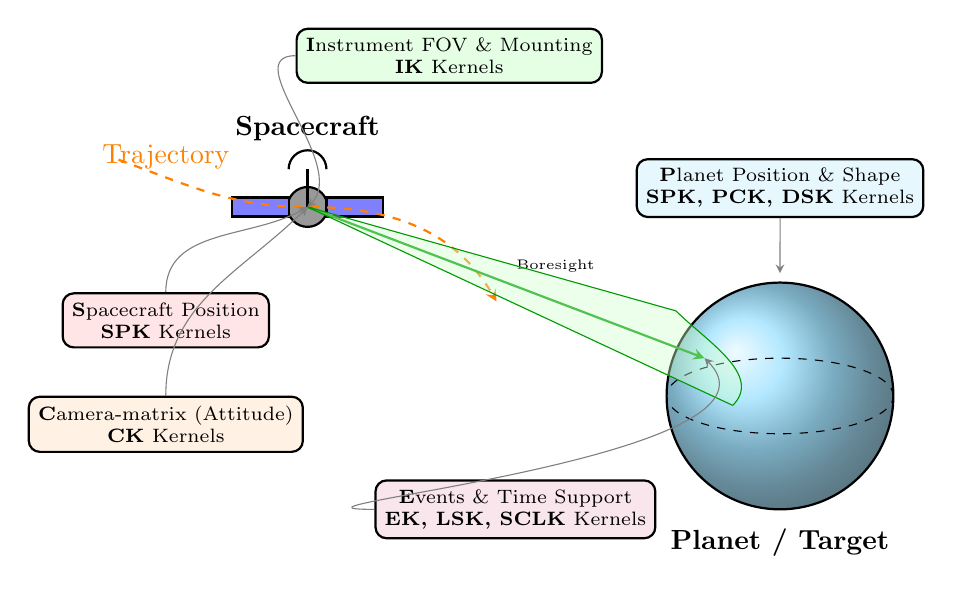
\begin{tikzpicture}[scale=1.2, >=stealth,
  lbl/.style={draw, fill=blue!5, rounded corners, font=\scriptsize, align=center, thick},
  title/.style={font=\bfseries}]

  % Draw Planet (P)
  \shade[ball color=blue!30!cyan!50, opacity=0.8] (5,0) circle (1.2cm);
  \draw[thick] (5,0) circle (1.2cm);
  \draw[dashed, thin] (5,0) ellipse (1.2cm and 0.4cm);
  \node[below, title] at (5,-1.3) {Planet / Target};
  
  % Draw Spacecraft (S)
  \coordinate (SC) at (0,2);
  \fill[gray!80] (SC) circle (6pt);
  \draw[thick] (SC) circle (6pt);
  % Solar panels
  \draw[thick, fill=blue!50] (-0.8, 1.9) rectangle (-0.2, 2.1);
  \draw[thick, fill=blue!50] (0.2, 1.9) rectangle (0.8, 2.1);
  % Antenna
  \draw[thick] (SC) -- (0, 2.4);
  \draw[thick] (-0.2, 2.4) arc (180:0:0.2);
  \node[above, title] at (0, 2.6) {Spacecraft};

  % Trajectory path (SPK)
  \draw[dashed, ->, orange, thick] (-2, 2.5) to[out=-20, in=180] (SC) to[out=0, in=120] (2, 1);
  \node[orange, above] at (-1.5, 2.3) {Trajectory};

  % Instrument (I) mounting & pointing cone
  \coordinate (Inst) at (0.1, 1.8);
  % Pointing vector / boresight to Planet surface
  \coordinate (TargetPt) at (4.2, 0.4);
  \draw[thick, ->, green!60!black] (SC) -- (TargetPt) node[midway, above right, black, font=\tiny] {Boresight};
  % Field of View (FOV) cone
  \fill[green!20, opacity=0.4] (SC) -- (3.9, 0.9) to[out=-45, in=45] (4.5, -0.1) -- cycle;
  \draw[green!60!black, thin] (SC) -- (3.9, 0.9);
  \draw[green!60!black, thin] (SC) -- (4.5, -0.1);
  \draw[green!60!black, thin] (3.9, 0.9) to[out=-45, in=45] (4.5, -0.1);

  % Acronym Blocks / Annotations
  \node[lbl, fill=red!10] (S_lbl) at (-1.5, 0.8) {{\bf S}pacecraft Position\\{\bf SPK} Kernels};
  \node[lbl, fill=orange!10] (C_lbl) at (-1.5, -0.3) {{\bf C}amera-matrix (Attitude)\\{\bf CK} Kernels};
  \node[lbl, fill=green!10] (I_lbl) at (1.5, 3.6) {{\bf I}nstrument FOV \& Mounting\\{\bf IK} Kernels};
  \node[lbl, fill=cyan!10] (P_lbl) at (5, 2.2) {{\bf P}lanet Position \& Shape\\{\bf SPK, PCK, DSK} Kernels};
  \node[lbl, fill=purple!10] (E_lbl) at (2.2, -1.2) {{\bf E}vents \& Time Support\\{\bf EK, LSK, SCLK} Kernels};

  % Connective lines from labels to graphics
  \draw[->, thin, gray] (S_lbl) to[out=90, in=210] (SC);
  \draw[->, thin, gray] (C_lbl) to[out=90, in=225] (SC);
  \draw[->, thin, gray] (I_lbl) to[out=180, in=45] (SC);
  \draw[->, thin, gray] (P_lbl) to[out=270, in=90] (5, 1.3);
  \draw[->, thin, gray] (E_lbl) to[out=180, in=315] (TargetPt);

\end{tikzpicture}
\end{center}
\FigCap{Conceptual overview of observation geometry and corresponding NASA SPICE kernels. The logical acronym {\bf SPICE} maps the physical components of an observation: {\bf S}pacecraft trajectory (SPK), {\bf P}lanet ephemeris and physical models (SPK/PCK/DSK), {\bf I}nstrument mounting and FOV parameters (IK), {\bf C}-matrix attitude (CK), and {\bf E}vents and time scale conversions (EK/LSK/SCLK). Supporting reference frames are defined in the Frame Kernel (FK).}
\end{figure}

This review aims to bridge this gap by providing a comprehensive, mathematically rigorous survey of the analytical models and numerical algorithms driving the SPICE toolkit. We detail the mechanical and geometric transformations that convert raw astronomical observables and instrument telemetry into high-precision scientific coordinate systems. We structure the paper as follows: Section 2 dissects the trajectory and ephemeris models of the SPK component. Section 3 reviews the rotational dynamics and body shape formulations of the PCK component. Section 4 presents the quaternion algebra and coordinate chain mathematics of the CK component. Section 5 evaluates the relativistic time system conversions. Finally, Section 6 explores the scientific consequences, providing quantitative analyses of error propagation, light-time correction, stellar aberration, shape model distortions, and numerical truncation limits.

\section{Ephemeris \& Trajectory Models (SPK Component)}
The SPK (Spacecraft and Planet Kernel) component is responsible for representing the position and velocity (state vector) of celestial bodies, spacecraft, and instruments as a function of time. SPICE stores these trajectories in discrete blocks within binary kernels and evaluates them continuously using two primary mathematical methodologies: numerical Chebyshev polynomial interpolation and analytical Keplerian propagation.

\subsection{Chebyshev Polynomial Interpolation}
For high-precision ephemerides (such as the JPL DE440 solar system ephemerides), storing raw position and velocity coordinates at high temporal resolution is computationally prohibitive. Instead, SPICE stores coefficients of Chebyshev polynomials of the first kind ($T_n(x)$) and interpolates them dynamically. 

Chebyshev polynomials are defined on the interval $x \in [-1, 1]$ by the trigonometric relation:
\begin{equation}
T_n(x) = \cos(n \arccos x)
\end{equation}
and satisfy the standard three-term recurrence relation:
\begin{align}
T_0(x) &= 1 \\
T_1(x) &= x \\
T_{n+1}(x) &= 2x T_n(x) - T_{n-1}(x)
\end{align}

To interpolate the state vector $(\mathbf{r}, \mathbf{v})$ at an arbitrary Ephemeris Time $t$ (seconds past the J2000 epoch) within a specific kernel interval $[t_{\text{start}}, t_{\text{end}}]$, SPICE first maps the physical time $t$ to the normalized domain $x \in [-1, 1]$ via the linear transformation:
\begin{equation}
x = \frac{2t - (t_{\text{start}} + t_{\text{end}})}{t_{\text{end}} - t_{\text{start}}}
\end{equation}

The position vector $\mathbf{r}(x) = [X(x), Y(x), Z(x)]^T$ is evaluated using a linear combination of Chebyshev polynomials of degree $N$:
\begin{equation}
\mathbf{r}(x) = \sum_{i=0}^N \mathbf{c}_i T_i(x)
\end{equation}
where $\mathbf{c}_i = [c_{x,i}, c_{y,i}, c_{z,i}]^T$ are the pre-computed Chebyshev coefficients stored in the SPK file.

Crucially, to maintain physical consistency and avoid numerical differentiation noise, SPICE evaluates the velocity vector $\mathbf{v}(t) = [V_x(t), V_y(t), V_z(t)]^T$ analytically rather than numerically. The velocity is obtained by applying the chain rule:
\begin{equation}
\mathbf{v}(t) = \frac{d\mathbf{r}(x)}{dx} \cdot \frac{dx}{dt} = \frac{2}{t_{\text{end}} - t_{\text{start}}} \sum_{i=1}^N \mathbf{c}_i T'_i(x)
\end{equation}
The derivatives of the Chebyshev polynomials $T'_i(x)$ are computed using the recurrence relation:
\begin{align}
T'_0(x) &= 0 \\
T'_1(x) &= 1 \\
T'_{n+1}(x) &= 2 T_n(x) + 2x T'_n(x) - T'_{n-1}(x)
\end{align}

The choice of Chebyshev polynomials is mathematically optimal due to the Chebyshev equioscillation theorem (minimax property). It guarantees that the maximum interpolation error is minimized over the interval, effectively suppressing Runge's phenomenon which plagues standard polynomial interpolation.

\subsection{Analytical Two-Body Keplerian Propagators}
For simplified orbits or initial mission planning phases, SPICE supports analytical orbital propagation using two-body conic elements (SPK Type 8 and 9). The classical Keplerian orbital elements consist of: semi-major axis $a$, eccentricity $e$, inclination $i$, longitude of the ascending node $\Omega$, argument of periapsis $\omega$, and mean anomaly $M_0$ at epoch $t_0$.

To propagate the state to a target time $t$, SPICE first computes the mean anomaly $M(t)$:
\begin{equation}
M(t) = M_0 + n(t - t_0)
\end{equation}
where $n = \sqrt{\mu / a^3}$ is the mean motion and $\mu$ is the gravitational parameter of the primary body. The eccentric anomaly $E(t)$ is solved numerically from the transcendental Kepler's Equation:
\begin{equation}
M(t) = E(t) - e \sin E(t)
\end{equation}
SPICE solves this equation using an iterative Newton-Raphson scheme:
\begin{equation}
E_{k+1} = E_k - \frac{E_k - e \sin E_k - M}{1 - e \cos E_k}
\end{equation}
converging rapidly within $4$ to $5$ iterations down to machine precision.

Once $E(t)$ is obtained, the position $\mathbf{r}_{\text{orb}}$ and velocity $\mathbf{v}_{\text{orb}}$ in the orbital plane (with the $x$-axis pointing towards periapsis) are:
\begin{equation}
\mathbf{r}_{\text{orb}} = \begin{pmatrix} a(\cos E - e) \\ a\sqrt{1-e^2}\sin E \\ 0 \end{pmatrix}, \quad
\mathbf{v}_{\text{orb}} = \frac{\sqrt{\mu a}}{r} \begin{pmatrix} -\sin E \\ \sqrt{1-e^2}\cos E \\ 0 \end{pmatrix}
\end{equation}
where the radial distance $r$ is $r = a(1 - e\cos E)$.

Finally, the state is transformed from the orbital plane coordinates to the target inertial reference frame by applying the standard 3-D rotation matrix $R(\Omega, i, \omega)$:
\begin{equation}
\mathbf{r} = R_z(-\Omega) R_x(-i) R_z(-\omega) \mathbf{r}_{\text{orb}}
\end{equation}
where $R_j(\theta)$ represents a standard passive rotation matrix about coordinate axis $j$.

\subsection{Numerical Integration and Relativistic Ephemerides}
For massive solar system bodies, SPICE coordinates are derived from the numerical integration of the relativistic Einstein-Infeld-Hoffmann (EIH) equations of motion, which account for multi-body Newtonian gravity and first-order post-Newtonian (1PN) relativistic corrections:
\begin{equation}
\mathbf{\ddot{r}}_i = \sum_{j \neq i} \frac{\mu_j (\mathbf{r}_j - \mathbf{r}_i)}{r_{ij}^3} + \mathbf{a}_{i,\text{PN}}
\end{equation}
where $\mathbf{a}_{i,\text{PN}}$ includes post-Newtonian terms representing gravitational time dilation and spatial curvature. The discrete state outputs of these massive integrations (e.g., JPL's DE440 ephemerides) are read by SPICE using Hermite interpolation (SPK Type 14) or high-degree Chebyshev polynomials to ensure that the relativistic orbits are reconstructed with sub-millimeter precision. In high-precision orbit determination of near-Earth objects and planetary crossers, these relativistic integrations and multi-body gravitational models are crucial for tracing close encounters and evaluating long-term dynamical stabilities (Sitarski 2002).

\section{Rotational Dynamics and Body Shape Models (PCK Component)}
To convert positions from an inertial frame (e.g., J2000) to a body-fixed, rotating frame (e.g., planetographic coordinates), SPICE utilizes the PCK (Physical Constants Kernel). PCK contains the mathematical parameters defining the orientation and physical dimensions of celestial bodies.

\subsection{Euler Angles and IAU Rotational Models}
The orientation of a celestial body's body-fixed frame relative to the J2000 inertial frame is defined by the three time-dependent Euler angles specified by the International Astronomical Union (IAU) (Archinal \etal 2018): right ascension ($\alpha_0, \dot{\alpha}$) and declination ($\delta_0, \dot{\delta}$) of the body's north pole, and the rotation angle of its prime meridian ($W_0, \dot{W}$). 

These angles are modeled as trigonometric series of time:
\begin{align}
\alpha(T) &= \alpha_0 + \dot{\alpha} T + \sum_i a_i \sin(\theta_i) \\
\delta(T) &= \delta_0 + \dot{\delta} T + \sum_i d_i \cos(\theta_i) \\
W(d) &= W_0 + \dot{W} d + \sum_i w_i \sin(\theta_i)
\end{align}
where $T$ is the time in Julian centuries of $36525$ days from the J2000.0 epoch ($T = \text{ET}/3155760000$), $d$ is the interval in days from the J2000.0 epoch ($d = \text{ET}/86400$), and $\theta_i$ represents long-period astronomical arguments (such as the mean anomalies of the planets or the Moon's node).

The rotation matrix $R_{\text{inertial}\rightarrow\text{body}}$ that transforms a position vector from the J2000 inertial frame to the body-fixed frame is constructed by chaining three consecutive rotations:
\begin{equation}
R_{\text{inertial}\rightarrow\text{body}} = R_z(W) R_x(90^\circ - \delta) R_z(90^\circ + \alpha)
\end{equation}

By expanding this matrix product, the complete coordinate transformation is:
\begin{equation}
\text{\footnotesize $
R_{\text{inertial}\rightarrow\text{body}} = 
\begin{pmatrix}
-\sin W \sin \alpha - \cos W \cos \alpha \sin \delta & \sin W \cos \alpha - \cos W \sin \alpha \sin \delta & \cos W \cos \delta \\
-\cos W \sin \alpha + \sin W \cos \alpha \sin \delta & \cos W \cos \alpha + \sin W \sin \alpha \sin \delta & -\sin W \cos \delta \\
\cos \alpha \cos \delta & \sin \alpha \cos \delta & \sin \delta
\end{pmatrix}
$}
\end{equation}

\subsection{Triaxial Ellipsoids vs. Digital Shape Models}
For large, hydrostatic equilibrium bodies (like major planets), SPICE models the physical surface as a triaxial ellipsoid defined by the quadratic equation:
\begin{equation}
\frac{x^2}{a^2} + \frac{y^2}{b^2} + \frac{z^2}{c^2} = 1
\end{equation}
where $a, b,$ and $c$ are the equatorial and polar semi-axes.

Astronomical coordinate mapping distinguishes between two types of latitudes on these ellipsoidal surfaces:
\begin{enumerate}
\item {\bf Planetocentric Latitude ($\phi_c$):} The angle between the position vector $\mathbf{r} = [x, y, z]^T$ and the equatorial plane:
\begin{equation}
\tan \phi_c = \frac{z}{\sqrt{x^2 + y^2}}
\end{equation}
\item {\bf Planetographic Latitude ($\phi_g$):} The angle between the outward surface normal vector $\mathbf{n}$ and the equatorial plane. The surface normal $\mathbf{n}$ at any point on the ellipsoid is computed via the gradient of the surface function:
\begin{equation}
\mathbf{n} = \nabla \left( \frac{x^2}{a^2} + \frac{y^2}{b^2} + \frac{z^2}{c^2} \right) = \begin{pmatrix} 2x/a^2 \\ 2y/b^2 \\ 2z/c^2 \end{pmatrix}
\end{equation}
For a spheroid ($a=b$), the relation between the latitudes simplifies to:
\begin{equation}
\tan \phi_g = \frac{a^2}{c^2} \tan \phi_c
\end{equation}
\end{enumerate}

\begin{figure}[htb]
\begin{center}
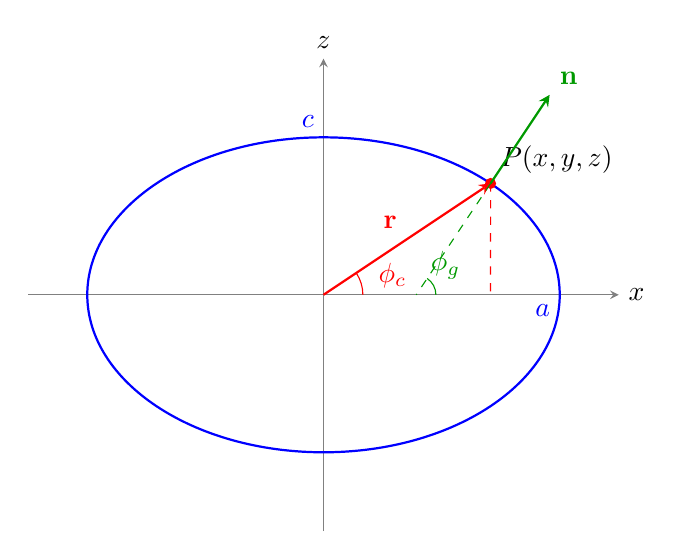
\begin{tikzpicture}[scale=2.5, >=stealth]
  % Draw axes
  \draw[->, gray, thin] (-1.5, 0) -- (1.5, 0) node[right, black] {$x$};
  \draw[->, gray, thin] (0, -1.2) -- (0, 1.2) node[above, black] {$z$};
  
  % Draw ellipse (spheroid outline) with a=1.2, b=0.8
  \draw[thick, blue] (0,0) ellipse (1.2cm and 0.8cm);
  
  % Define point P on the ellipse at angle 45 degrees in parameter t
  % x = a cos(t) = 1.2 * cos(45) = 0.8485
  % z = b sin(t) = 0.8 * sin(45) = 0.5657
  \coordinate (P) at (0.8485, 0.5657);
  
  % Draw position vector r
  \draw[thick, ->, red] (0,0) -- (P) node[midway, above left] {$\mathbf{r}$};
  \fill[red] (P) circle (0.8pt) node[above right, black] {$P(x,y,z)$};
  
  % Draw line for planetocentric latitude angle phi_c
  \draw[dashed, red] (P) -- (0.8485, 0);
  \draw[red, thin] (0.2, 0) arc (0:33.69:0.2);
  \node[red] at (0.35, 0.1) {$\phi_c$};
  
  % Calculate normal vector normal n at P
  % n_x = x/a^2 = 0.8485/1.44 = 0.589
  % n_z = z/b^2 = 0.5657/0.64 = 0.884
  % Normal starts at P and goes to P + (0.3, 0.45) = (1.15, 1.02)
  \coordinate (N_end) at (1.1485, 1.0157);
  \draw[thick, ->, green!60!black] (P) -- (N_end) node[above right] {$\mathbf{n}$};
  
  % Surface normal extended backwards to intersect x-axis
  % Equation of normal line: z - z_p = (n_z/n_x) * (x - x_p)
  % Slope = n_z/n_x = 0.884/0.589 = 1.5
  % Intersection with z=0: x_int = x_p - z_p/1.5 = 0.8485 - 0.5657/1.5 = 0.471
  \coordinate (X_int) at (0.471, 0);
  \draw[dashed, green!60!black] (P) -- (X_int);
  
  % Draw planetographic latitude angle phi_g
  \draw[green!60!black, thin] (0.571, 0) arc (0:56.30:0.1);
  \node[green!60!black] at (0.62, 0.15) {$\phi_g$};
  
  % Bounding box label
  \node[blue, below left] at (1.2, 0) {$a$};
  \node[blue, above left] at (0, 0.8) {$c$};
  
\end{tikzpicture}
\end{center}
\FigCap{Planetocentric latitude $\phi_c$ vs. planetographic latitude $\phi_g$ on an oblate spheroid representing a celestial body's reference ellipsoid. The position vector $\mathbf{r}$ defines $\phi_c$, whereas the surface normal $\mathbf{n}$ defines $\phi_g$, satisfying the differential relation $\tan\phi_g = \frac{a^2}{c^2}\tan\phi_c$.}
\end{figure}

For irregular bodies such as comets and small asteroids, the smooth ellipsoidal model fails completely. SPICE supports Digital Shape Kernels (DSK) to model irregular geometries using two mathematical representations: tessellated plate-vertex meshes (DSK Type 2) and digital elevation models (DSK Type 4) (Pajusalu \etal 2022). 

A tessellated plate mesh represents the body as a set of $V$ vertices $\mathbf{V}_i \in \mathbb{R}^3$ and $P$ triangular plates $P_j = (\mathbf{v}_{j,1}, \mathbf{v}_{j,2}, \mathbf{v}_{j,3})$ where $\mathbf{v}_{j,k}$ are references to the vertex set. 

A primary mathematical task in observational astronomy is finding the intersection of an instrument's boresight ray with the body's surface. A ray is parameterized as:
\begin{equation}
\mathbf{r}(t) = \mathbf{p}_0 + t \mathbf{\hat{d}}, \quad t \ge 0
\end{equation}
where $\mathbf{p}_0$ is the ray origin (e.g., spacecraft position) and $\mathbf{\hat{d}}$ is the unit direction vector of the boresight. To determine if this ray intersects a triangular plate, SPICE implements the Möller-Trumbore ray-triangle intersection algorithm, which bypasses the costly computation of the plane equation. 

Let $\mathbf{E}_1 = \mathbf{v}_2 - \mathbf{v}_1$ and $\mathbf{E}_2 = \mathbf{v}_3 - \mathbf{v}_1$ be the edges of the triangle. The intersection point must satisfy:
\begin{equation}
\mathbf{p}_0 + t \mathbf{\hat{d}} = (1 - u - v)\mathbf{v}_1 + u\mathbf{v}_2 + v\mathbf{v}_3
\end{equation}
which is rearranged as a system of linear equations:
\begin{equation}
\begin{pmatrix} -\mathbf{\hat{d}} & \mathbf{E}_1 & \mathbf{E}_2 \end{pmatrix} \begin{pmatrix} t \\ u \\ v \end{pmatrix} = \mathbf{p}_0 - \mathbf{v}_1
\end{equation}

By defining $\mathbf{T} = \mathbf{p}_0 - \mathbf{v}_1$, $\mathbf{P} = \mathbf{\hat{d}} \times \mathbf{E}_2$, and $\mathbf{Q} = \mathbf{T} \times \mathbf{E}_1$, Cramer's rule yields the solution:
\begin{equation}
\begin{pmatrix} t \\ u \\ v \end{pmatrix} = \frac{1}{\mathbf{P} \cdot \mathbf{E}_1} \begin{pmatrix} \mathbf{Q} \cdot \mathbf{E}_2 \\ \mathbf{P} \cdot \mathbf{T} \\ \mathbf{Q} \cdot \mathbf{\hat{d}} \end{pmatrix}
\end{equation}
An intersection occurs if and only if $t \ge 0$, $u \ge 0$, $v \ge 0$, and $u + v \le 1$. To handle millions of plates efficiently, SPICE constructs spatial octrees or bounding volume hierarchies (BVH) inside DSK files, reducing the ray-tracing search complexity from $\mathcal{O}(P)$ to $\mathcal{O}(\log P)$ (Xystouris \etal 2024).

\section{Coordinate Transformations \& Quaternion Mathematics (CK Component)}
Spacecraft attitude (orientation) telemetry is highly dynamic due to active attitude control systems. In SPICE, these rotations are stored in CK (C-matrix Kernel) files using four-dimensional unit quaternions.

\subsection{Quaternions for Attitude Representation}
To represent the rotation of a coordinate frame, quaternions are numerically superior to Euler angles as they completely avoid gimbal lock (singularity at high inclinations) and require only four parameters instead of a nine-element matrix, reducing computational overhead and floating-point errors.

A unit quaternion $q$ is defined on the four-dimensional sphere $S^3$ as:
\begin{equation}
q = q_0 + q_1 \mathbf{i} + q_2 \mathbf{j} + q_3 \mathbf{k} = (q_0, \mathbf{q}_{\text{vec}})
\end{equation}
where $\mathbf{i}^2 = \mathbf{j}^2 = \mathbf{k}^2 = \mathbf{i}\mathbf{j}\mathbf{k} = -1$, and $||q||^2 = q_0^2 + q_1^2 + q_2^2 + q_3^2 = 1$. The scalar part $q_0$ and vector part $\mathbf{q}_{\text{vec}}$ represent a rotation of angle $\theta$ about a unit axis $\mathbf{\hat{u}}$:
\begin{equation}
q_0 = \cos\left(\frac{\theta}{2}\right), \quad \mathbf{q}_{\text{vec}} = \sin\left(\frac{\theta}{2}\right) \mathbf{\hat{u}}
\end{equation}

Astronomers must be highly cautious when interfacing with SPICE quaternions. SPICE uses a unique convention that differs from the standard Hamilton quaternion product. Let $p$ and $q$ be two quaternions. The SPICE quaternion product $p *_{\text{SPICE}} q$ is defined as:
\begin{equation}
p *_{\text{SPICE}} q = \begin{pmatrix} p_0 q_0 - \mathbf{p}_{\text{vec}} \cdot \mathbf{q}_{\text{vec}} \\ p_0 \mathbf{q}_{\text{vec}} + q_0 \mathbf{p}_{\text{vec}} - \mathbf{p}_{\text{vec}} \times \mathbf{q}_{\text{vec}} \end{pmatrix}
\end{equation}
Note the minus sign before the cross product. This definition is the conjugate of the standard Hamilton product (which uses $+ \mathbf{p}_{\text{vec}} \times \mathbf{q}_{\text{vec}}$). This specific convention is chosen so that the multiplication order of attitude quaternions matches the multiplication order of the corresponding rotation matrices:
\begin{equation}
R(p *_{\text{SPICE}} q) = R(p) \cdot R(q)
\end{equation}
The rotation matrix $R(q)$ associated with a SPICE unit quaternion $q$ is:
\begin{equation}
R(q) = \begin{pmatrix} 
1 - 2(q_2^2 + q_3^2) & 2(q_1 q_2 - q_0 q_3) & 2(q_1 q_3 + q_0 q_2) \\ 
2(q_1 q_2 + q_0 q_3) & 1 - 2(q_1^2 + q_3^2) & 2(q_2 q_3 - q_0 q_1) \\ 
2(q_1 q_3 - q_0 q_2) & 2(q_2 q_3 + q_0 q_1) & 1 - 2(q_1^2 + q_2^2) 
\end{pmatrix}
\end{equation}

\subsection{Quaternion Interpolation (SLERP)}
Spacecraft orientation is telemetry-derived and sampled discretely. To find the orientation at an arbitrary time $t$ between two discrete samples $q(t_1) = q_1$ and $q(t_2) = q_2$, SPICE implements Spherical Linear Interpolation (SLERP).

SLERP computes the shortest path along the great circle on the 3-sphere $S^3$, preserving the constant angular velocity of the rotation. The SLERP formula is:
\begin{equation}
\text{Slerp}(q_1, q_2; \tau) = \frac{\sin((1-\tau)\theta)}{\sin\theta} q_1 + \frac{\sin(\tau\theta)}{\sin\theta} q_2
\end{equation}
where $\tau = (t - t_1)/(t_2 - t_1) \in [0, 1]$ is the normalized interpolation parameter, and $\theta$ is the angular sweep between the two quaternions:
\begin{equation}
\cos\theta = q_1 \cdot q_2 = q_{1,0}q_{2,0} + q_{1,1}q_{2,1} + q_{1,2}q_{2,2} + q_{1,3}q_{2,3}
\end{equation}

If $\cos\theta < 0$, the quaternion $q_2$ is replaced by $-q_2$ to ensure that the interpolation traverses the shortest path (since $q$ and $-q$ represent the same physical orientation). If $\theta \to 0$ (highly aligned quaternions), the formula becomes numerically unstable due to the division by $\sin\theta$. SPICE handles this case by transitioning to standard normalized linear interpolation (LERP):
\begin{equation}
\text{Slerp}(q_1, q_2; \tau) \approx \frac{(1-\tau)q_1 + \tau q_2}{||(1-\tau)q_1 + \tau q_2||}
\end{equation}

\subsection{SPICE Reference Frame Classification (FK Component)}
To manage the orientations and origins of diverse celestial and artificial bodies, SPICE classifies reference frames based on their kinematic characteristics. Mathematically, a reference frame $F$ is defined as a coordinate origin (center) $\mathbf{O}(t)$ and a right-handed orthonormal basis vectors $\{ \mathbf{e}_x(t), \mathbf{e}_y(t), \mathbf{e}_z(t) \}$ in $\mathbb{R}^3$, satisfying:
\begin{equation}
\mathbf{e}_i \cdot \mathbf{e}_j = \delta_{ij}, \quad \mathbf{e}_x \times \mathbf{e}_y = \mathbf{e}_z
\end{equation}
SPICE groups these reference frames into five major classes defined in the Frame Kernel (FK) component (Acton \etal 2018):
\begin{enumerate}
\item {\bf Inertial Reference Frames:} Non-rotating coordinate systems whose axes point in fixed directions relative to distant stars. Crucially, the origin $\mathbf{O}(t)$ has negligible acceleration ($\ddot{\mathbf{O}}(t) \approx \mathbf{0}$) relative to the cosmic rest frame, and the basis vectors are time-invariant ($\dot{\mathbf{e}}_i = \mathbf{0}$). In SPICE, the center of all inertial frames is physically placed at the Solar System Barycenter (SSB) to ensure Newtonian equations of motion hold without fictitious force terms. Examples include the Earth equatorial standard J2000 (EME2000), the ecliptic standard ECLIPJ2000, and the International Celestial Reference Frame (ICRF).
\item {\bf Body-Fixed Frames (PCK):} Non-inertial, rotating coordinate systems attached to the center of mass of a celestial body (e.g., major planets, natural satellites, asteroids). The origin is coincident with the body's center ($\mathbf{O}_{\text{body}}(t)$), and the axes rotate continuously with the body. Their time-varying orientation relative to inertial space is modeled via rotational elements (Right Ascension $\alpha$, Declination $\delta$, and Prime Meridian orientation $W$) defined in Physical Constants Kernels (PCK).
\item {\bf Spacecraft \& Instrument Frames (CK/IK):} Non-inertial coordinate systems centered at the center of mass of a spacecraft or at the focal/mounting center of an instrument sensor. These axes are highly dynamic, with orientations determined by high-rate attitude control telemetry (stored in C-matrix Kernels, CK) or static alignment offsets (stored in Instrument Kernels, IK).
\item {\bf Topocentric Frames (FK):} Coordinate systems centered at a specific landing site, radar antenna, or geographical station $\mathbf{O}_{\text{site}}(t)$ on a body's surface. The basis is defined geodetically: the $\mathbf{e}_z$ axis is aligned with the local outward ellipsoid surface normal (zenith), while $\mathbf{e}_x$ and $\mathbf{e}_y$ axes point toward local East and North.
\item {\bf Dynamic Frames (FK):} Coordinate systems whose basis vectors are computed dynamically as a function of time based on astronomical vectors (e.g., the Earth-Sun vector, spacecraft velocity vector, or angular momentum vector).
\end{enumerate}

These frames form a directed tree structure where each node is a coordinate frame and each edge represents a coordinate transformation matrix. Figure 3 illustrates this relational frame hierarchy.

\begin{figure}[htb]
\begin{center}
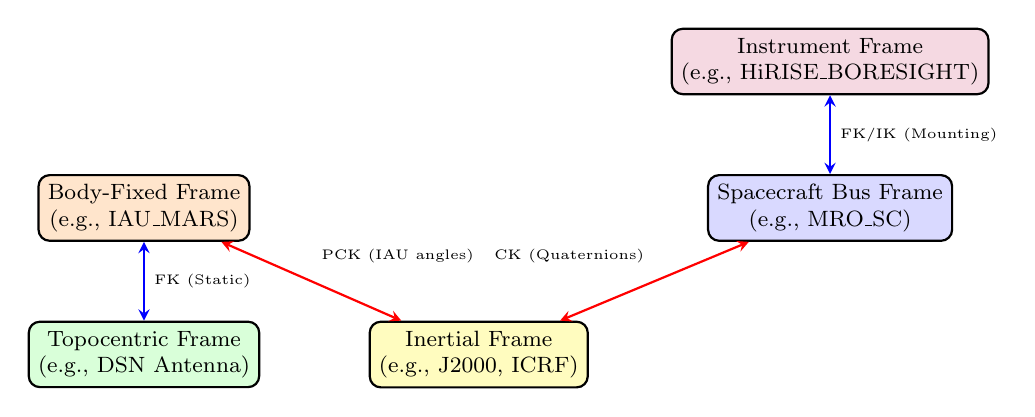
\begin{tikzpicture}[node distance=1.0cm and 1.5cm, >=stealth, 
  block/.style={rectangle, draw, fill=blue!10, rounded corners, minimum width=2.6cm, minimum height=0.8cm, align=center, thick},
  font=\footnotesize]
  
  % Nodes
  \node[block, fill=yellow!25] (Inertial) at (0,0) {Inertial Frame\\(e.g., J2000, ICRF)};
  
  \node[block, fill=orange!20] (PCK) [above left=of Inertial] {Body-Fixed Frame\\(e.g., IAU\_MARS)};
  \node[block, fill=blue!15] (CK) [above right=of Inertial] {Spacecraft Bus Frame\\(e.g., MRO\_SC)};
  \node[block, fill=green!15] (Topo) [below=of PCK] {Topocentric Frame\\(e.g., DSN Antenna)};
  \node[block, fill=purple!15] (Inst) [above=of CK] {Instrument Frame\\(e.g., HiRISE\_BORESIGHT)};

  % Paths / Edges
  \draw[<->, thick, red] (PCK) -- (Inertial) node[midway, above right, black, font=\tiny, yshift=0.1cm] {PCK (IAU angles)};
  \draw[<->, thick, red] (CK) -- (Inertial) node[midway, above left, black, font=\tiny, yshift=0.1cm] {CK (Quaternions)};
  \draw[<->, thick, blue] (PCK) -- (Topo) node[midway, right, black, font=\tiny] {FK (Static)};
  \draw[<->, thick, blue] (CK) -- (Inst) node[midway, right, black, font=\tiny] {FK/IK (Mounting)};
  
\end{tikzpicture}
\nobreak
\end{center}
\FigCap{Structural hierarchy and coordinate frame transitions in the NASA SPICE system. The central hub is the Barycentric Inertial frame (ICRF/J2000). Transitions to rotating celestial bodies are modeled via the PCK (IAU orientation angles), transitions to spacecraft are modeled via the CK (attitude quaternions), and local mounting structures or topographic landing sites are linked via Frame and Instrument Kernels (FK and IK).}
\end{figure}

\subsubsection{The Primary Inertial Standard: J2000 vs. ICRF}
In observational astrometry and deep-space navigation, the choice of the primary inertial standard determines the foundational coordinate system upon which all subsequent kinematic chains are anchored. The SPICE toolkit relies on the J2000 frame (historically known as Earth Mean Equator and Equinox of J2000 or EME2000) as its primary inertial reference (Acton \etal 2018). As illustrated in Figure 4, the J2000 frame is defined based on the Earth's precessional and orbital kinematics:
\begin{itemize}
\item The origin $\mathbf{O}_{\text{J2000}}(t)$ is centered at the Solar System Barycenter (SSB) (or the center of mass of Earth for geocentric formulations).
\item The $+Z_{\text{J2000}}$ axis is aligned normal to the Earth's mean equatorial plane at the epoch J2000 (noon on 2000 January 01 TDB / JD $2451545.0$).
\item The $+X_{\text{J2000}}$ axis points along the mean vernal equinox ($\Upsilon$), which is defined by the intersection of the mean equatorial plane and the ecliptic plane (Earth's orbital plane) at the J2000 epoch.
\item The $+Y_{\text{J2000}}$ axis completes the right-handed orthonormal triad: $\mathbf{e}_y = \mathbf{e}_z \times \mathbf{e}_x$.
\end{itemize}

\begin{figure}[htb]
\begin{center}
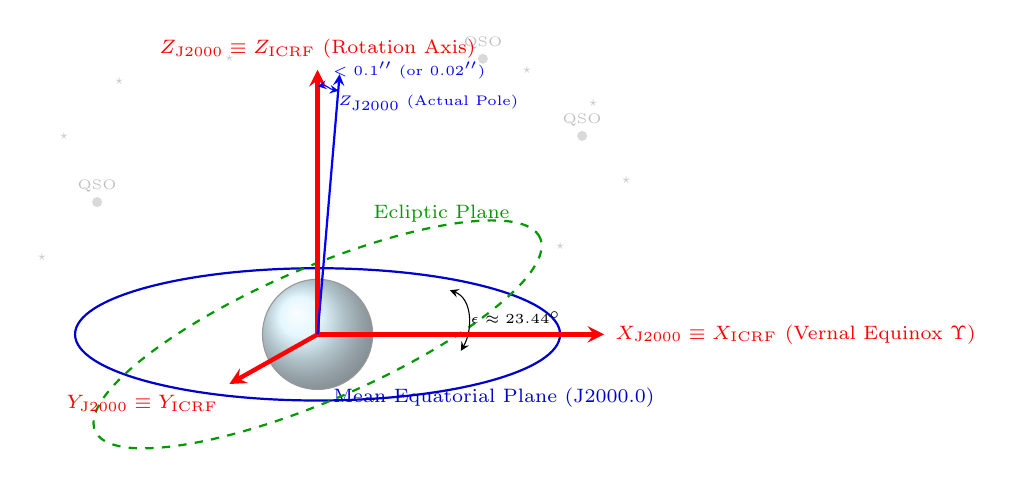
\begin{tikzpicture}[scale=1.4, >=stealth]

  % Draw background star field representing ICRF
  \foreach \p in {(2.5,2.1), (2.8,1.4), (2.2,0.8), (1.9,2.4), (-2.3,1.8), (-1.8,2.3), (-2.5,0.7), (0.5,2.6), (-0.8,2.5)} {
    \node[gray!40, font=\tiny] at \p {$\star$};
  }
  \foreach \q in {(2.4,1.8), (-2.0,1.2), (1.5,2.5)} {
    \draw[gray!30, fill=gray!30] \q circle (0.04); % Quasar representation
    \node[gray!50, above, font=\tiny] at \q {QSO};
  }

  % Draw Earth at origin
  \shade[ball color=blue!30!cyan!20, opacity=0.7] (0,0) circle (0.5cm);
  \draw[gray!80, thin] (0,0) circle (0.5cm);

  % Draw equatorial plane (slanted ellipse)
  \draw[thick, blue!80!black] (0,0) ellipse (2.2cm and 0.6cm);
  \node[blue!80!black, below, font=\scriptsize] at (1.6,-0.4) {Mean Equatorial Plane (J2000.0)};

  % Draw ecliptic plane (inclined by 23.44 deg)
  \begin{scope}[rotate=23.44]
    \draw[thick, green!60!black, dashed] (0,0) ellipse (2.2cm and 0.6cm);
    \node[green!60!black, above, font=\scriptsize] at (1.4,0.4) {Ecliptic Plane};
  \end{scope}

  % Draw Earth's obliquity angle arc
  \draw[<->, thin] (1.3, -0.15) to[out=60, in=-20] (1.2, 0.4);
  \node[right, font=\tiny] at (1.3, 0.15) {$\epsilon \approx 23.44^\circ$};

  % Reference Frame Axes
  % X-axis: pointing to vernal equinox
  \draw[->, ultra thick, red] (0,0) -- (2.6, 0) node[anchor=west, font=\scriptsize] {$X_{\text{J2000}} \equiv X_{\text{ICRF}}$ (Vernal Equinox $\Upsilon$)};

  % Z-axis: rigid kinematic axis (defined by quasar positions)
  \draw[->, ultra thick, red] (0,0) -- (0, 2.4) node[anchor=south, font=\scriptsize] {$Z_{\text{J2000}} \equiv Z_{\text{ICRF}}$ (Rotation Axis)};

  % Y-axis: completes right-handed system
  \draw[->, ultra thick, red] (0,0) -- (-0.8, -0.45) node[anchor=north east, font=\scriptsize] {$Y_{\text{J2000}} \equiv Y_{\text{ICRF}}$};

  % Illustrate the tiny difference between J2000 and ICRF (exaggerated for visibility)
  \draw[->, blue, thick] (0,0) -- (0.2, 2.36);
  \node[blue, right, font=\tiny] at (0.1, 2.1) {$Z_{\text{J2000}}$ (Actual Pole)};
  \draw[<->, thin, blue] (0,2.25) to[out=10, in=170] (0.19, 2.21);
  \node[above right, blue, font=\tiny] at (0.05, 2.23) {$< 0.1''$ (or $0.02''$)};

\end{tikzpicture}
\end{center}
\FigCap{The J2000 and International Celestial Reference Frame (ICRF) alignment. The J2000 coordinate system is physically defined by the Earth's mean equator (historically referred to as EME2000) and mean equinox at epoch J2000.0 (noon on 2000 Jan 01 TDB). The ICRF is a kinematic frame defined by radio-frequency positions of hundreds of distant quasars (QSOs). In SPICE, the frame label {\tt "J2000"} is treated as mathematically equivalent to the high-precision ICRF, with their axes aligned to within $0.02''$. The blue vector illustrates the actual physical J2000 Earth equator normal relative to the rigid ICRF frame.}
\end{figure}

In modern high-precision astrometry, the International Astronomical Union (IAU) has replaced dynamically-defined frames with the International Celestial Reference Frame (ICRF). The ICRF is realized through the Very Long Baseline Interferometry (VLBI) observations of hundreds of extragalactic radio sources (mostly quasars). Because these quasars are billions of light-years away, they have no detectable proper motion ($< 10\ \mu\text{as/yr}$), making the ICRF an exceptionally stable and rigid kinematic reference that is completely independent of Earth's orbital and precessional wobbles.

To preserve optical compatibility, the axes of the ICRF were aligned to match the optical J2000.0 frame as closely as possible. The residual rotational offset between the two frames is less than $0.02$ arcseconds, which is well within the optical measurement uncertainty of the J2000 epoch. In the SPICE toolkit, this micro-arcsecond offset is far below standard observation precision thresholds. Therefore, to ensure historical compatibility and avoid costly runtime matrix evaluations:
\begin{enumerate}
\item SPICE uses the string label {\tt "J2000"} to access its primary inertial frame.
\item Under the hood, any kernel data or coordinate vectors specified relative to {\tt "J2000"} are physically referenced directly to the {\bf ICRF}.
\item SPICE treats {\tt "J2000"} and {\tt "ICRF"} as mathematically identical. No rotation matrix is evaluated when transitioning between J2000 and ICRF, preserving computational efficiency while delivering VLBI-level stability.
\end{enumerate}

\subsection{Coordinate System Conventions and Mathematical Mappings}
While a reference frame defines the orientation of physical axes and the location of the origin, a {\it coordinate system} defines the mathematical methodology used to locate a point in space relative to that frame (Acton \etal 2018). SPICE supports several key coordinate systems to facilitate planetary science and mission geometry. Figure 5 illustrates these conventions on a single point $P(x,y,z)$.

\begin{figure}[htb]
\begin{center}
\begin{tikzpicture}[scale=1.5, >=stealth,
  axis/.style={->,thick},
  vector/.style={->,thick,red},
  projection/.style={dashed,blue},
  angle/.style={->,thin,draw=black!70,font=\tiny}]

  % Draw coordinate axes
  \draw[axis] (0,0,0) -- (2.5,0,0) node[anchor=north]{$x$ (Prime Meridian)};
  \draw[axis] (0,0,0) -- (0,2.5,0) node[anchor=south]{$z$ (Rotation Axis)};
  \draw[axis] (0,0,0) -- (0,0,3.5) node[anchor=north east]{$y$};

  % Define Point P
  \coordinate (O) at (0,0,0);
  \coordinate (P) at (0.777, 1.555, 1.347);
  \coordinate (ProjXY) at (0.777, 0, 1.347); % Projection in equatorial plane

  % Draw vector OP
  \draw[vector] (O) -- (P) node[anchor=south west] {$P(x,y,z)$};

  % Draw projections
  \draw[projection] (P) -- (ProjXY);
  \draw[projection] (O) -- (ProjXY);
  \draw[projection] (P) -- (0, 1.555, 0) node[left, black, font=\tiny] {$z$};
  \draw[projection] (ProjXY) -- (0.777, 0, 0) node[below, black, font=\tiny] {$x$};
  \draw[projection] (ProjXY) -- (0, 0, 1.347) node[below left, black, font=\tiny] {$y$};

  % Label range (r)
  \node[red, above left, font=\scriptsize] at (0.35, 0.75, 0.6) {$r$};

  % Label cylindrical radius (rho)
  \node[blue, below right, font=\scriptsize] at (0.4, 0, 0.8) {$\rho$};

  % Draw Angles
  % Longitude (lambda) - in equatorial plane
  \draw[angle] (0.5,0,0) to[out=-20, in=120] (0.3,0,0.5);
  \node[below, font=\scriptsize] at (0.35, 0, 0.25) {$\lambda$};

  % Latitude (phi) - angle from ProjXY to OP
  \draw[angle] (0.6,0,1.0) to[out=90, in=-20] (0.5,0.8,0.8);
  \node[right, font=\scriptsize] at (0.55, 0.45, 0.85) {$\phi$};

  % Co-latitude (theta) - angle from Z axis to OP
  \draw[angle] (0,0.6,0) to[out=0, in=80] (0.3,0.5,0.2);
  \node[above right, font=\scriptsize] at (0.1, 0.65, 0.15) {$\theta$};

\end{tikzpicture}
\end{center}
\FigCap{SPICE Coordinate System Conventions. A point $P$ can be represented using: (1) Cartesian rectangular coordinates $(x,y,z)$; (2) Planetocentric latitudinal coordinates $(r,\phi,\lambda)$ with distance $r$, latitude $\phi$, and longitude $\lambda$; (3) Spherical coordinates $(r,\theta,\lambda)$ using co-latitude $\theta$; or (4) Cylindrical coordinates $(\rho,\lambda,z)$ with cylindrical radius $\rho$ in the equatorial plane.}
\end{figure}

The mathematical formulations and forward/inverse conversion mappings implemented in the SPICE subroutine library are detailed below:

\begin{enumerate}
\item {\bf Cartesian (Rectangular) Coordinates:} Evaluated as $(x, y, z) \in \mathbb{R}^3$, representing orthogonal spatial offsets relative to the origin along the frame's basis axes.
\item {\bf Planetocentric Latitudinal Coordinates:} Represented as $(r, \phi, \lambda)$, where $r \in [0, \infty)$ is the range (distance to origin), $\phi \in [-\pi/2, \pi/2]$ is the planetocentric latitude (angle measured northward from the equatorial plane), and $\lambda \in [0, 2\pi)$ is the longitude (measured positive eastward from the prime meridian).
The conversion from Cartesian to Latitudinal coordinates (implemented in {\tt reclat\_c}) is derived as:
\begin{align}
r &= \sqrt{x^2 + y^2 + z^2} \\
\phi &= \arcsin\left(\frac{z}{r}\right) \\
\lambda &= \text{atan2}(y, x) \pmod{2\pi}
\end{align}
The inverse conversion from Latitudinal to Cartesian coordinates (implemented in {\tt latrec\_c}) is:
\begin{align}
x &= r \cos\phi \cos\lambda \\
y &= r \cos\phi \sin\lambda \\
z &= r \sin\phi
\end{align}

\item {\bf Spherical Coordinates:} Represented as $(r, \theta, \lambda)$, where $r \in [0, \infty)$ is the range, $\theta \in [0, \pi]$ is the co-latitude or polar angle (measured downward from the positive $z$-axis), and $\lambda \in [0, 2\pi)$ is the longitude.
The conversion from Cartesian to Spherical coordinates (implemented in {\tt recsph\_c}) is:
\begin{align}
r &= \sqrt{x^2 + y^2 + z^2} \\
\theta &= \arccos\left(\frac{z}{r}\right) \\
\lambda &= \text{atan2}(y, x) \pmod{2\pi}
\end{align}
The inverse conversion (implemented in {\tt sphrec\_c}) is:
\begin{align}
x &= r \sin\theta \cos\lambda \\
y &= r \sin\theta \sin\lambda \\
z &= r \cos\theta
\end{align}

\item {\bf Cylindrical Coordinates:} Represented as $(\rho, \lambda, z)$, where $\rho \in [0, \infty)$ is the cylindrical radius (perpendicular distance from the $z$-axis), $\lambda \in [0, 2\pi)$ is the longitude, and $z$ is the axial height.
The conversion from Cartesian to Cylindrical coordinates (implemented in {\tt reccyl\_c}) is:
\begin{align}
\rho &= \sqrt{x^2 + y^2} \\
\lambda &= \text{atan2}(y, x) \pmod{2\pi} \\
z &= z
\end{align}
The inverse conversion (implemented in {\tt cylrec\_c}) is:
\begin{align}
x &= \rho \cos\lambda \\
y &= \rho \sin\lambda \\
z &= z
\end{align}

\item {\bf Planetographic Coordinates:} Represented as $(h, \phi_g, \lambda_g)$, where $h$ is the height above the reference ellipsoid, $\phi_g$ is the planetographic latitude (the angle between the surface normal vector and the equatorial plane), and $\lambda_g$ is the planetographic longitude.
To maintain consistency with historic maps, SPICE enforces a unique longitude convention (the IAU 2000 standard) for planetographic coordinates. For prograde rotating celestial bodies (which rotate counter-clockwise when viewed from the north pole, such as Earth or Mars), the planetographic longitude increases positively {\it westward} (opposite to the body's rotation). For retrograde rotating bodies (such as Venus), the longitude increases positively {\it eastward}. This convention ensures that for an observer standing on the surface of any body, the longitude of the sub-observer point increases monotonically with time. Cartesian conversions are computed iteratively using ellipsoidal coordinate mappings (via {\tt recpgr\_c} and {\tt pgrrec\_c}), taking into account the equatorial radius $a$ and flattening factor $f$:
\begin{equation}
f = \frac{a - c}{a}
\end{equation}
\end{enumerate}

\subsection{Chaining Transformations}
To visually and mathematically map how SPICE links an instrument's sensor frame to the global celestial standard (inertial space), we construct the core Chain of Vector Transformations. In the absence of target-specific coordinates or light-time aberrations, a vector $\mathbf{R}_{\text{Instrument}}$ in the sensor frame is mapped to the standard inertial frame (e.g., J2000 or ICRF) as:
\begin{equation}
\mathbf{R}_{\text{Inertial}} = \mathbf{M}_{\text{FK}} \cdot \mathbf{M}_{\text{CK}}(t) \cdot \mathbf{M}_{\text{Offset}} \cdot \mathbf{R}_{\text{Instrument}}
\end{equation}
where:
\begin{itemize}
\item $\mathbf{R}_{\text{Instrument}}$ is the raw pixel/boresight vector.
\item $\mathbf{M}_{\text{Offset}}$ is the static orientation matrix accounting for mounting misalignment (stored in the Instrument Kernel, IK).
\item $\mathbf{M}_{\text{CK}}(t)$ is the time-dependent spacecraft rotation matrix derived from attitude telemetry (stored in the C-Kernel, CK).
\item $\mathbf{M}_{\text{FK}}$ is the structural frame kernel matrix aligning the local system to the celestial inertial standard (defined in the Frame Kernel, FK).
\end{itemize}

Further extending this chain to convert an observation vector from the instrument's sensor frame to a target planet's body-fixed coordinate system requires chaining target-relative calculations and evaluating each time-dependent matrix at its correct relativistic epoch:
\begin{equation}
\mathbf{v}_{\text{target}}(t_{\text{emit}}) = R_{\text{inertial}\rightarrow\text{body}}(t_{\text{emit}}) \cdot R_{\text{sc}\rightarrow\text{inertial}}(t_{\text{recv}}) \cdot R_{\text{inst}\rightarrow\text{sc}} \cdot \mathbf{v}_{\text{inst}}
\end{equation}
where:
\begin{itemize}
\item $R_{\text{inst}\rightarrow\text{sc}}$ is the static rotation matrix from the instrument frame to the spacecraft body frame (obtained from the I-K).
\item $R_{\text{sc}\rightarrow\text{inertial}}(t_{\text{recv}})$ is the time-dependent spacecraft orientation evaluated at the receive time $t_{\text{recv}}$ (obtained from the C-Kernel, CK).
\item $R_{\text{inertial}\rightarrow\text{body}}(t_{\text{emit}})$ is the orientation of the target body evaluated at the emission time $t_{\text{emit}} = t_{\text{recv}} - \Delta t_{\text{lt}}$ (obtained from the PCK).
\end{itemize}

This matrix chain represents the fundamental algebraic structure of astrometric observation geometry, ensuring that the light-time delay ($\Delta t_{\text{lt}}$) is correctly accounted for at each stage of the coordinate conversion.

\subsection{Frame Tree Pathfinding and State Transformations (pxform vs. sxform)}
Under the hood, SPICE does not simply apply hardcoded formulas for every frame pair; instead, it implements a generalized graph-theoretic pathfinder. The database of coordinate systems is modeled as a directed tree (the ``Frame Tree'') where each node is a reference frame and each directed edge represents a known, immediate parent-child transformation. 

To convert coordinates from an arbitrary source frame $A$ to a target frame $B$ at an epoch $t$, SPICE searches the tree to find the unique, shortest path connecting the two nodes:
\begin{equation}
A = F_0 \longleftrightarrow F_1 \longleftrightarrow \dots \longleftrightarrow F_n = B
\end{equation}
The search traces the lineage of both frames back to their nearest common ancestor node (which is typically a fundamental inertial standard such as J2000 or ICRF). For each step $i$ along this path, SPICE evaluates the 3x3 coordinate rotation matrix:
\begin{equation}
M_{i \to i+1}^*(t) = \begin{cases} 
M_{F_i \to F_{i+1}}(t), & \text{if traversing from child to parent (upwards)} \\
M_{F_{i+1} \to F_i}^T(t), & \text{if traversing from parent to child (downwards)} 
\end{cases}
\end{equation}
Chaining these matrices via ordered matrix multiplication yields the overall position transformation matrix $R_{A \to B}(t)$, which is returned by the core SPICE routine {\tt pxform\_c}:
\begin{equation}
R_{A \to B}(t) = M_{n-1 \to n}^*(t) \cdots M_{1 \to 2}^*(t) M_{0 \to 1}^*(t)
\end{equation}

Astronomers must distinguish between transforming static positions and dynamic velocities. For a 3-dimensional position vector $\mathbf{r}_A$, the transition is simple:
\begin{equation}
\mathbf{r}_B(t) = R_{A \to B}(t) \mathbf{r}_A(t)
\end{equation}
However, if we are transforming a 6-dimensional state vector $\mathbf{s}_A = [\mathbf{r}_A, \mathbf{v}_A]^T$ containing both position and velocity, the derivative of the coordinate rotation matrix $\dot{R}(t)$ must be included to account for Coriolis and centrifugal accelerations between rotating frames. The transformed velocity is:
\begin{equation}
\mathbf{v}_B(t) = R_{A \to B}(t) \mathbf{v}_A(t) + \dot{R}_{A \to B}(t) \mathbf{r}_A(t)
\end{equation}
This is represented as a 6x6 block-matrix multiplication, returned by the SPICE routine {\tt sxform\_c}:
\begin{equation}
\begin{pmatrix} \mathbf{r}_B(t) \\ \mathbf{v}_B(t) \end{pmatrix} = S_{A \to B}(t) \begin{pmatrix} \mathbf{r}_A(t) \\ \mathbf{v}_A(t) \end{pmatrix} \quad \text{where} \quad S_{A \to B}(t) = \begin{pmatrix} R_{A \to B}(t) & \mathbf{0}_{3\times 3} \\ \dot{R}_{A \to B}(t) & R_{A \to B}(t) \end{pmatrix}
\end{equation}

For dynamic frames (such as CK spacecraft or PCK rotating bodies), the instantaneous relative angular velocity vector $\boldsymbol{\omega}(t) = [\omega_x, \omega_y, \omega_z]^T$ is read from kernels or calculated from analytical models. The time derivative $\dot{R}(t)$ is then computed analytically via the kinematic relation:
\begin{equation}
\dot{R}(t) = -[\boldsymbol{\omega}(t)]_{\times} R(t)
\end{equation}
where $[\boldsymbol{\omega}(t)]_{\times}$ is the skew-symmetric cross-product matrix:
\begin{equation}
[\boldsymbol{\omega}(t)]_{\times} = \begin{pmatrix} 0 & -\omega_z & \omega_y \\ \omega_z & 0 & -\omega_x \\ -\omega_y & \omega_x & 0 \end{pmatrix}
\end{equation}
When chaining multiple rotating frames, state transformation matrices are chained using 6x6 matrix multiplication:
\begin{equation}
S_{A \to C}(t) = S_{B \to C}(t) \cdot S_{A \to B}(t) = \begin{pmatrix} R_{BC} R_{AB} & \mathbf{0}_{3\times 3} \\ \dot{R}_{BC} R_{AB} + R_{BC} \dot{R}_{AB} & R_{BC} R_{AB} \end{pmatrix}
\end{equation}
which automatically incorporates the chain rule on matrix derivatives, preserving exact physical velocities throughout arbitrary observational geometries.

\section{Time System Conversions (The ``E'' Component)}
Time in astronomy is highly non-linear due to general and special relativity and the Earth's variable rotation. SPICE's ``E'' (Events) component provides the mathematical machinery to convert between diverse time scales, utilizing continuous relativistic corrections.

\subsection{Astronomical Time Scales}
SPICE operates internally on Ephemeris Time (ET), which is defined as the number of barycentric dynamical seconds past the J2000.0 epoch. Mathematically, ET is equivalent to Barycentric Dynamical Time (TDB). The relationships between key astronomical time scales are:
\begin{enumerate}
\item {\bf Coordinated Universal Time (UTC):} A civil time scale based on atomic clocks (TAI) but kept within $0.9$ seconds of Earth's rotational time (UT1) by inserting leap seconds ($\Delta t_{\text{leap}}$).
\item {\bf International Atomic Time (TAI):} A continuous, highly stable atomic time scale.
\item {\bf Terrestrial Time (TT):} An idealized coordinate time scale on the Earth's geoid:
\begin{equation}
TT = TAI + 32.184\text{ s}
\end{equation}
\item {\bf Barycentric Dynamical Time (TDB):} A coordinate time scale defined at the Solar System Barycenter (SSB), reflecting relativistic effects.
\end{enumerate}

\subsection{Relativistic Time Differentials}
Converting from Terrestrial Time (TT) to Barycentric Dynamical Time (TDB) requires correcting for the gravitational redshift and time dilation experienced by an Earth-bound observer relative to the Solar System Barycenter. This correction is known as the Einstein delay (or relativistic time differential).

SPICE implements a highly optimized analytical model developed by JPL to compute this differential:
\begin{equation}
TDB - TT = 0.001657 \sin(g) + 0.000022 \sin(2g)
\end{equation}
where $g$ is the mean anomaly of the Earth-Moon barycenter around the Sun:
\begin{equation}
g = 357.529191^\circ + 35999.050290^\circ T
\end{equation}
and $T$ is the number of Julian centuries past the J2000 epoch.

The peak-to-peak amplitude of this relativistic differential is approximately $1.65$ milliseconds. While seemingly small, a time error of $1.65$ milliseconds at the orbital speed of the Earth ($\approx 29.78\text{ km/s}$) corresponds to a spatial position error of approximately $49\text{ meters}$, which is unacceptable for modern spacecraft ranging and astrometric observations.

The complete transformation from UTC to Ephemeris Time (ET) is thus given by:
\begin{equation}
ET = UTC + \Delta t_{\text{leap}} + 32.184 + 0.001657 \sin(g) + 0.000022 \sin(2g)
\end{equation}
where $\Delta t_{\text{leap}}$ is obtained dynamically from the SPICE leapseconds kernel (LSK).

\section{The Geometry Finder (GF) Subsystem: Numerical Root-Finding and Event Search}
While SPICE is widely utilized for forward calculations---interpolating spacecraft positions or body orientations at a specific epoch---it also contains a powerful backward solver known as the {\it Geometry Finder} (GF) subsystem. The GF subsystem allows scientists and mission designers to identify time intervals during which specific geometric conditions are satisfied (Acton \etal 2018). Examples include occultations, distance extrema (periapsis/apoapsis), coordinate range crossings, and ray-body surface intersections.

\subsection{SPICE Windows and Set Arithmetic}
At the core of the GF subsystem is the mathematical concept of a {\it SPICE Window}. Analytically, a window $W$ is defined as a union of a finite number of disjoint, closed intervals of ephemeris time (ET):
\begin{equation}
W = \bigcup_{i=1}^{N} [t_{2i-1}, t_{2i}], \quad \text{where } t_1 < t_2 < \dots < t_{2N}
\end{equation}
To search for events, a user provides a {\it confinement window} $W_{\text{conf}}$ representing the overall time domain of interest. The GF solver computes a {\it result window} $W_{\text{res}} \subseteq W_{\text{conf}}$ containing only the intervals during which the geometric condition is met. SPICE implements a suite of rigorous double-precision set arithmetic operations (such as union $W_A \cup W_B$, intersection $W_A \cap W_B$, and complement $W^c$) to allow complex, multi-variable logical queries (e.g., finding intervals where a spacecraft is in Mars' shadow {\it and} the target instrument is pointed within $5^\circ$ of a specific landing site).

\subsection{The Dual-Pass Search Engine}
Evaluating non-linear, transcendental physical equations (e.g., finding the exact epoch when the angular distance between two bodies reaches a local minimum) requires a highly robust numerical search framework. To guarantee that no events are missed while achieving sub-millisecond precision, the GF subsystem employs a dual-pass numerical engine:
\begin{enumerate}
\item {\bf Pass 1: Bracketing (Grid Search):} The confinement window $W_{\text{conf}}$ is sampled at discrete, uniformly spaced epochs $t_k = t_0 + k \Delta t_{\text{step}}$. The algorithm evaluates the state of the target geometric function $f(t)$ at each step to check for a sign change:
\begin{equation}
f(t_k) \cdot f(t_{k+1}) \leq 0
\end{equation}
When a sign change is detected, a state boundary is successfully bracketed within the interval $[t_k, t_{k+1}]$.
\item {\bf Pass 2: Convergence and Refinement (Root-Finding):} Once a transition is bracketed, the solver executes a root-finding algorithm to locate the exact transition epoch $t^*$ such that:
\begin{equation}
|f(t^*) - y_{\text{target}}| < \epsilon_{\text{tol}}
\end{equation}
where $\epsilon_{\text{tol}}$ is a user-specified convergence tolerance (typically $10^{-6}$ seconds or less).
\end{enumerate}

\subsection{Numerical Caveats and Temporal Aliasing}
Because SPICE models orientational precessions, irregular shape meshes, and relativistic orbital dynamics, analytical derivatives $f'(t)$ are generally unavailable. Therefore, the second-pass root-finder utilizes a modified {\it Brent's method}---a stable, derivative-free numerical root-finder that dynamically combines the bisection method, the secant method, and inverse quadratic interpolation. 

A critical pitfall in the GF subsystem is the selection of the first-pass step size $\Delta t_{\text{step}}$. If $\Delta t_{\text{step}}$ is chosen larger than the duration of the event (or half the period of $f(t)$), the bracketing algorithm will fail to detect any sign changes, completely bypassing the event. This is a classic temporal aliasing/under-sampling problem. To ensure numerical reliability, astronomers must satisfy the sampling condition:
\begin{equation}
\Delta t_{\text{step}} < \Delta t_{\text{event}}
\end{equation}
where $\Delta t_{\text{event}}$ is the shortest expected duration of the target event. Selecting $\Delta t_{\text{step}}$ requires balancing computational cost (which scales as $\mathcal{O}(1/\Delta t_{\text{step}})$) with the physical scales of the dynamics under study.

\section{The Astronomy Pivot: Scientific Consequences and Error Propagation}
A major pitfall in observational astronomy is neglecting the physical and numerical error propagation associated with the mathematical models implemented in SPICE. In this section, we quantify the errors introduced by using simplified geometric models.

\subsection{Light-Time and Stellar Aberration Corrections}
When analyzing observations of a celestial target, scientists must choose between three levels of aberration correction:
\begin{enumerate}
\item {\bf Geometric State (No Correction):} The position of the target at the observer's epoch $t_{\text{recv}}$.
\item {\bf Light-Time Correction:} Accounts for the finite speed of light ($c$). The target position is evaluated at the emission epoch $t_{\text{emit}} = t_{\text{recv}} - \Delta t_{\text{lt}}$. The light-time equation is transcendental:
\begin{equation}
\Delta t_{\text{lt}} = \frac{||\mathbf{r}_{\text{target}}(t_{\text{recv}} - \Delta t_{\text{lt}}) - \mathbf{r}_{\text{obs}}(t_{\text{recv}})||}{c}
\end{equation}
SPICE solves this iteratively:
\begin{equation}
\Delta t_{\text{lt}}^{(k+1)} = \frac{||\mathbf{r}_{\text{target}}(t_{\text{recv}} - \Delta t_{\text{lt}}^{(k)}) - \mathbf{r}_{\text{obs}}(t_{\text{recv}})||}{c}
\end{equation}
converging to sub-millisecond accuracy within $3$ iterations.
\item {\bf Stellar Aberration Correction:} Accounts for the relative velocity of the observer $\mathbf{v}_{\text{obs}}$ relative to the Solar System Barycenter. By applying special relativity, the apparent direction unit vector $\mathbf{\hat{u}}'$ is:
\begin{equation}
\mathbf{\hat{u}}' = \frac{\mathbf{\hat{u}} + \mathbf{v}_{\text{obs}}/c + (\gamma - 1)(\mathbf{\hat{u}} \cdot \mathbf{\hat{v}}_{\text{obs}}) \mathbf{\hat{v}}_{\text{obs}}}{1 + \mathbf{\hat{u}} \cdot \mathbf{v}_{\text{obs}}/c}
\end{equation}
where $\gamma = 1/\sqrt{1 - v_{\text{obs}}^2/c^2}$. In the low-velocity limit, this simplifies to the classical aberration formula:
\begin{equation}
\mathbf{\hat{u}}' \approx \mathbf{\hat{u}} + \frac{\mathbf{v}_{\text{obs}} - (\mathbf{\hat{u}} \cdot \mathbf{v}_{\text{obs}})\mathbf{\hat{u}}}{c}
\end{equation}
\end{enumerate}

\begin{figure}[htb]
\begin{center}
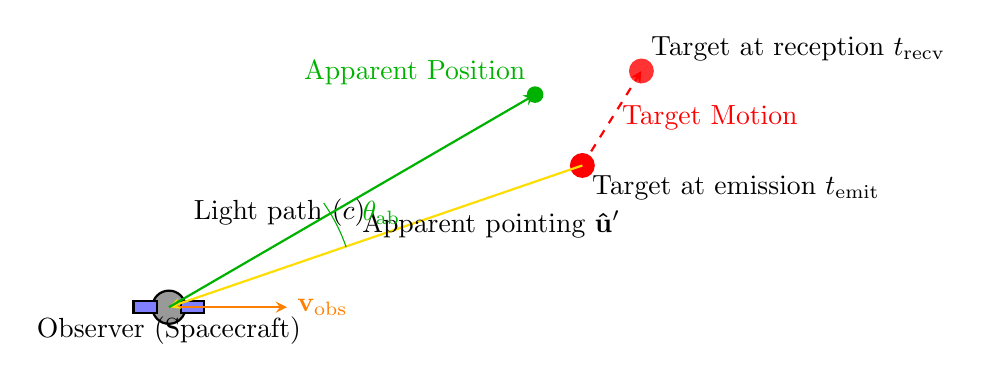
\begin{tikzpicture}[scale=1.5, >=stealth]
  % Spacecraft / Observer at (0,0)
  \coordinate (Obs) at (0,0);
  \fill[gray!80] (Obs) circle (4pt);
  \draw[thick] (Obs) circle (4pt);
  % Solar panels of spacecraft
  \draw[thick, fill=blue!50] (-0.3, -0.05) rectangle (-0.1, 0.05);
  \draw[thick, fill=blue!50] (0.1, -0.05) rectangle (0.3, 0.05);
  \node[below] at (Obs) {Observer (Spacecraft)};
  
  % Observer velocity vector v_obs
  \draw[thick, ->, orange] (Obs) -- (1, 0) node[right] {$\mathbf{v}_{\text{obs}}$};
  
  % Target true position at t_recv
  \coordinate (T_recv) at (4, 2);
  \fill[red!80] (T_recv) circle (3pt);
  \node[above right] at (T_recv) {Target at reception $t_{\text{recv}}$};
  
  % Target true position at t_emit
  \coordinate (T_emit) at (3.5, 1.2);
  \fill[red] (T_emit) circle (3pt);
  \node[below right] at (T_emit) {Target at emission $t_{\text{emit}}$};
  
  % Target motion vector
  \draw[->, thick, red, dashed] (T_emit) -- (T_recv) node[midway, right] {Target Motion};
  
  % Light path from T_emit to Obs
  \draw[thick, ->, yellow!80!orange] (T_emit) -- (Obs) node[midway, above left, black] {Light path ($c$)};
  
  % Apparent direction shifted by Stellar Aberration
  % The velocity of observer is to the right (x direction), which tilts the incoming light vector forward (towards x)
  % Apparent target position is shifted in the direction of v_obs
  \coordinate (T_app) at (3.1, 1.8);
  \draw[thick, ->, green!70!black] (Obs) -- (T_app) node[midway, below right, black] {Apparent pointing $\mathbf{\hat{u}}'$};
  \fill[green!70!black] (T_app) circle (2pt) node[above left] {Apparent Position};
  
  % Pointing shift angle (aberration)
  \draw[green!70!black, thin] (1.5, 0.51) arc (19:35:1.5);
  \node[green!70!black] at (1.8, 0.8) {$\theta_{\text{ab}}$};

\end{tikzpicture}
\end{center}
\FigCap{Geometrical representation of observational corrections in the SPICE toolkit. The target's position is corrected for light-time delay ($\Delta t_{\text{lt}}$) by evaluating its state at the emission epoch $t_{\text{emit}}$. The observer's velocity $\mathbf{v}_{\text{obs}}$ tilts the incoming light ray forward by the aberration angle $\theta_{\text{ab}}$, resulting in the apparent pointing direction $\mathbf{\hat{u}}'$.}
\end{figure}

\MakeTable{l c c c}{12.5cm}{Astrometric effects and observational errors at $1\text{ AU}$}
{\hline
Physical Effect & Mathematical Formulation & Peak Magnitude & Spatial Error at $1\text{ AU}$\\
\hline
Light-time delay & $\Delta t_{\text{lt}} = d/c$ & $\sim 499\text{ s}$ & $1.5 \times 10^8\text{ km}$ \\
Stellar aberration (Earth) & $\theta \approx v_{\text{obs}}/c$ & $20.496''$ & $1.49 \times 10^4\text{ km}$ \\
Stellar aberration (Mars) & $\theta \approx v_{\text{obs}}/c$ & $2.41''$ & $1.75 \times 10^3\text{ km}$ \\
Einstein delay (TDB $-$ TT) & $\Delta t_{\text{rel}} = 1.657\text{ ms} \sin g$ & $1.657\text{ ms}$ & $0.497\text{ km}$ \\
Obliquity nutation & IAU 1980 / 2000 Series & $9.21''$ & $6.7 \times 10^3\text{ km}$ \\
\hline
\multicolumn{4}{p{11.5cm}}{This table summarizes the main astrometric and relativistic effects computed in the SPICE toolkit, their peak angular magnitudes, and the equivalent spatial displacement at an astronomical unit ($1\text{ AU} \approx 1.496 \times 10^8\text{ km}$).}
}

As shown in Table 1, neglecting stellar aberration on Earth introduces a pointing error of $20.496''$ (arcseconds). For deep-space telescopes like the James Webb Space Telescope (JWST) or high-resolution imagers like HiRISE on the Mars Reconnaissance Orbiter (MRO), an error of this magnitude would cause the target to fall entirely outside the instrument's field of view, resulting in failed observations.

In real-world astrometric data reduction, these mathematical corrections must be applied to observational coordinates to prevent systematic offsets. Small observational errors and uncorrected stellar aberration directly map into severe orbital determination uncertainties. Tracing how these coordinate errors propagate into estimated orbital parameters is a major challenge in asteroid orbit refinement, particularly for potentially hazardous objects (Wlodarczyk 2015) and newly discovered asteroids where the observational arc is extremely short (Wlodarczyk \etal 2017).

\subsection{Geometric Body Shape Model Distortion}
Approximating a highly irregular body (like an asteroid or comet) as a triaxial ellipsoid introduces severe errors in mapping coordinates, calculating local slope angles, and estimating surface surface-area-to-volume ratios.

\MakeTable{l c c c}{12.5cm}{Physical characteristics and coordinate modeling errors for selected irregular bodies}
{\hline
Celestial Target & Mean Dimensions (km) & Shape Model Type & Max. Positional/Normal Discrepancy\\
\hline
101955 Bennu & $0.565 \times 0.543 \times 0.508$ & Triaxial Ellipsoid & $\Delta h \approx 36\text{ m}$, $\Delta \theta_n \approx 32^\circ$ \\
& Tessellated Plate Mesh & DSK (Type 2) & reference ($\sim 0.1\text{ m}$ accuracy) \\
162173 Ryugu & $1.00 \times 0.99 \times 0.89$ & Triaxial Ellipsoid & $\Delta h \approx 28\text{ m}$, $\Delta \theta_n \approx 28^\circ$ \\
& Tessellated Plate Mesh & DSK (Type 2) & reference ($\sim 0.1\text{ m}$ accuracy) \\
67P/C-G & $4.10 \times 3.25 \times 1.30$ & Triaxial Ellipsoid & $\Delta h \approx 1.2\text{ km}$, $\Delta \theta_n \approx 85^\circ$ \\
& Tessellated Plate Mesh & DSK (Type 2) & reference ($\sim 0.5\text{ m}$ accuracy) \\
\hline
\multicolumn{4}{p{11.5cm}}{Comparison of triaxial ellipsoid approximations with high-resolution Digital Shape Kernels (DSK) for highly irregular bodies. $\Delta h$ represents the maximum radial elevation error, and $\Delta \theta_n$ represents the maximum surface normal angular discrepancy.}
}

Table 2 highlights these geometric errors for three targets: 101955 Bennu, 162173 Ryugu, and Comet 67P/Churyumov-Gerasimenko. For Comet 67P, which exhibits a highly irregular, bi-lobed shape, a triaxial ellipsoid approximation leads to a maximum elevation error ($\Delta h$) of $1.2\text{ km}$ and a surface normal error ($\Delta \theta_n$) of $85^\circ$. Using an ellipsoidal shape model for spacecraft proximity operations or instrument alignment on such bodies would be catastrophic, resulting in surface collision or instrument misalignment.

\subsection{Numerical Truncation and Quaternion Drift}
All SPICE calculations are performed using double-precision floating-point numbers (IEEE 754 standard), providing $53$ bits of precision ($\approx 15$-$17$ decimal digits). When chaining numerous coordinate transformations over long-duration planetary missions, small floating-point roundoff errors accumulate.

A major source of numerical drift is the loss of quaternion normalization. In theory, a rotation quaternion must have a norm of exactly $1$. However, successive multiplications and interpolations introduce floating-point errors, causing $||q|| \neq 1$. If a non-unit quaternion is converted to a rotation matrix, the resulting matrix is non-orthogonal:
\begin{equation}
R(q)^T R(q) \neq I
\end{equation}
This violates coordinate rigidity, causing physical distortion (stretching or shearing) of vectors. To prevent this, SPICE routinely re-normalizes quaternions ($q \leftarrow q/||q||$) and enforces orthogonality on all computed C-matrices by executing a Procrustes-like projection back to the special orthogonal group $SO(3)$. Without these mathematical corrections, numerical truncation would lead to systematic, arcsecond-level pointing errors on deep-space telescopes over multi-year cruise phases.

\section{Conclusions}
In this survey, we have systematically reviewed the mathematical models and algorithms underpinning NASA's SPICE toolkit, detailing the equations that govern trajectories (SPK), rotational dynamics (PCK), attitude kinematics (CK), and relativistic time scales (the ``E'' component). By shifting the perspective of SPICE from a simple software library to a rigorous analytical system, we have highlighted how astronomers can avoid geometric errors and coordinate distortions.

Our quantitative analysis of observational errors emphasizes that high-precision astrometry requires rigorous, post-Newtonian relativistic time scale conversions, detailed stellar aberration and light-time corrections, and highly resolved Digital Shape Kernels (DSK) for irregular bodies. As space missions target increasingly complex objects and demand ever-higher pointing resolutions, a deep, mathematically transparent understanding of observation geometry remains a critical prerequisite for scientific success in observational astronomy.

\Acknow{We express our gratitude to the Navigation and Ancillary Information Facility (NAIF) team at the Jet Propulsion Laboratory (JPL/NASA) for their long-term dedication to maintaining the SPICE system. We also thank the Nehru Institute of Technology for providing the research facilities and computational support necessary to complete this study.}

\begin{references}
\refitem{Acton, C.H.}{1996}{Planet. Space Sci.}{44}{65}
\refitem{Acton, C., Bachman, N., Semenov, B., and Wright, E.}{2018}{Planet. Space Sci.}{150}{9}
\refitem{Archinal, B.A., \etal}{2018}{Celest. Mech. Dyn. Astron.}{130}{22}
\refitem{Folkner, W.M., Williams, J.G., Boggs, D.H., Park, R.S., and Kuchynka, P.}{2014}{IPN Prog. Rep.}{42-196}{1}
\refitem{Lieske, J.H.}{1979}{Astron. Astrophys.}{73}{282}
\refitem{Miranda, E.}{2024}{Electronics}{13}{2480}
\refitem{Pajusalu, M., \etal}{2022}{PLoS ONE}{17}{e0263882}
\refitem{Seidelmann, P.K., \etal}{2007}{Celest. Mech. Dyn. Astron.}{98}{155}
\refitem{Sitarski, G.}{2002}{Acta Astron.}{52}{471}
\refitem{Standish, E.M.}{1998}{JPL IOM}{312.F-98-048}{1}
\refitem{Wlodarczyk, I.}{2015}{Acta Astron.}{65}{215}
\refitem{Wlodarczyk, I., Cernis, K., and Boyle, R.P.}{2017}{Acta Astron.}{67}{81}
\refitem{Xystouris, G., Shebanits, O., and Arridge, C.S.}{2024}{RAS Tech. Instrum.}{3}{166}
\end{references}

\end{document}
